% Options for packages loaded elsewhere
\PassOptionsToPackage{unicode}{hyperref}
\PassOptionsToPackage{hyphens}{url}
%
\documentclass[
  11pt,
  ignorenonframetext,
]{beamer}
\usepackage{pgfpages}
\setbeamertemplate{caption}[numbered]
\setbeamertemplate{caption label separator}{: }
\setbeamercolor{caption name}{fg=normal text.fg}
\beamertemplatenavigationsymbolsempty
% Prevent slide breaks in the middle of a paragraph
\widowpenalties 1 10000
\raggedbottom
\setbeamertemplate{part page}{
  \centering
  \begin{beamercolorbox}[sep=16pt,center]{part title}
    \usebeamerfont{part title}\insertpart\par
  \end{beamercolorbox}
}
\setbeamertemplate{section page}{
  \centering
  \begin{beamercolorbox}[sep=12pt,center]{part title}
    \usebeamerfont{section title}\insertsection\par
  \end{beamercolorbox}
}
\setbeamertemplate{subsection page}{
  \centering
  \begin{beamercolorbox}[sep=8pt,center]{part title}
    \usebeamerfont{subsection title}\insertsubsection\par
  \end{beamercolorbox}
}
\AtBeginPart{
  \frame{\partpage}
}
\AtBeginSection{
  \ifbibliography
  \else
    \frame{\sectionpage}
  \fi
}
\AtBeginSubsection{
  \frame{\subsectionpage}
}
\usepackage{amsmath,amssymb}
\usepackage{lmodern}
\usepackage{iftex}
\ifPDFTeX
  \usepackage[T1]{fontenc}
  \usepackage[utf8]{inputenc}
  \usepackage{textcomp} % provide euro and other symbols
\else % if luatex or xetex
  \usepackage{unicode-math}
  \defaultfontfeatures{Scale=MatchLowercase}
  \defaultfontfeatures[\rmfamily]{Ligatures=TeX,Scale=1}
\fi
\usetheme[]{metropolis}
% Use upquote if available, for straight quotes in verbatim environments
\IfFileExists{upquote.sty}{\usepackage{upquote}}{}
\IfFileExists{microtype.sty}{% use microtype if available
  \usepackage[]{microtype}
  \UseMicrotypeSet[protrusion]{basicmath} % disable protrusion for tt fonts
}{}
\makeatletter
\@ifundefined{KOMAClassName}{% if non-KOMA class
  \IfFileExists{parskip.sty}{%
    \usepackage{parskip}
  }{% else
    \setlength{\parindent}{0pt}
    \setlength{\parskip}{6pt plus 2pt minus 1pt}}
}{% if KOMA class
  \KOMAoptions{parskip=half}}
\makeatother
\usepackage{xcolor}
\newif\ifbibliography
\usepackage{graphicx}
\makeatletter
\def\maxwidth{\ifdim\Gin@nat@width>\linewidth\linewidth\else\Gin@nat@width\fi}
\def\maxheight{\ifdim\Gin@nat@height>\textheight\textheight\else\Gin@nat@height\fi}
\makeatother
% Scale images if necessary, so that they will not overflow the page
% margins by default, and it is still possible to overwrite the defaults
% using explicit options in \includegraphics[width, height, ...]{}
\setkeys{Gin}{width=\maxwidth,height=\maxheight,keepaspectratio}
% Set default figure placement to htbp
\makeatletter
\def\fps@figure{htbp}
\makeatother
\setlength{\emergencystretch}{3em} % prevent overfull lines
\providecommand{\tightlist}{%
  \setlength{\itemsep}{0pt}\setlength{\parskip}{0pt}}
\setcounter{secnumdepth}{-\maxdimen} % remove section numbering
\ifLuaTeX
  \usepackage{selnolig}  % disable illegal ligatures
\fi
\IfFileExists{bookmark.sty}{\usepackage{bookmark}}{\usepackage{hyperref}}
\IfFileExists{xurl.sty}{\usepackage{xurl}}{} % add URL line breaks if available
\urlstyle{same} % disable monospaced font for URLs
\hypersetup{
  pdftitle={Medidas de dispersión},
  pdfauthor={Gerardo Martín},
  hidelinks,
  pdfcreator={LaTeX via pandoc}}

\title{Medidas de dispersión}
\author{Gerardo Martín}
\date{2022-06-29}

\begin{document}
\frame{\titlepage}

\begin{frame}{¿Qué son?}
\protect\hypertarget{quuxe9-son}{}
\begin{itemize}
\item
  Descripción de la variabilidad de los datos:

  \begin{itemize}
  \tightlist
  \item
    Cuánto se alejan del promedio
  \item
    Diferencia entre máximo y mínimo
  \end{itemize}
\end{itemize}
\end{frame}

\hypertarget{cuxf3mo-se-llaman}{%
\section{¿Cómo se llaman?}\label{cuxf3mo-se-llaman}}

\begin{frame}{``\,''}
\protect\hypertarget{section}{}
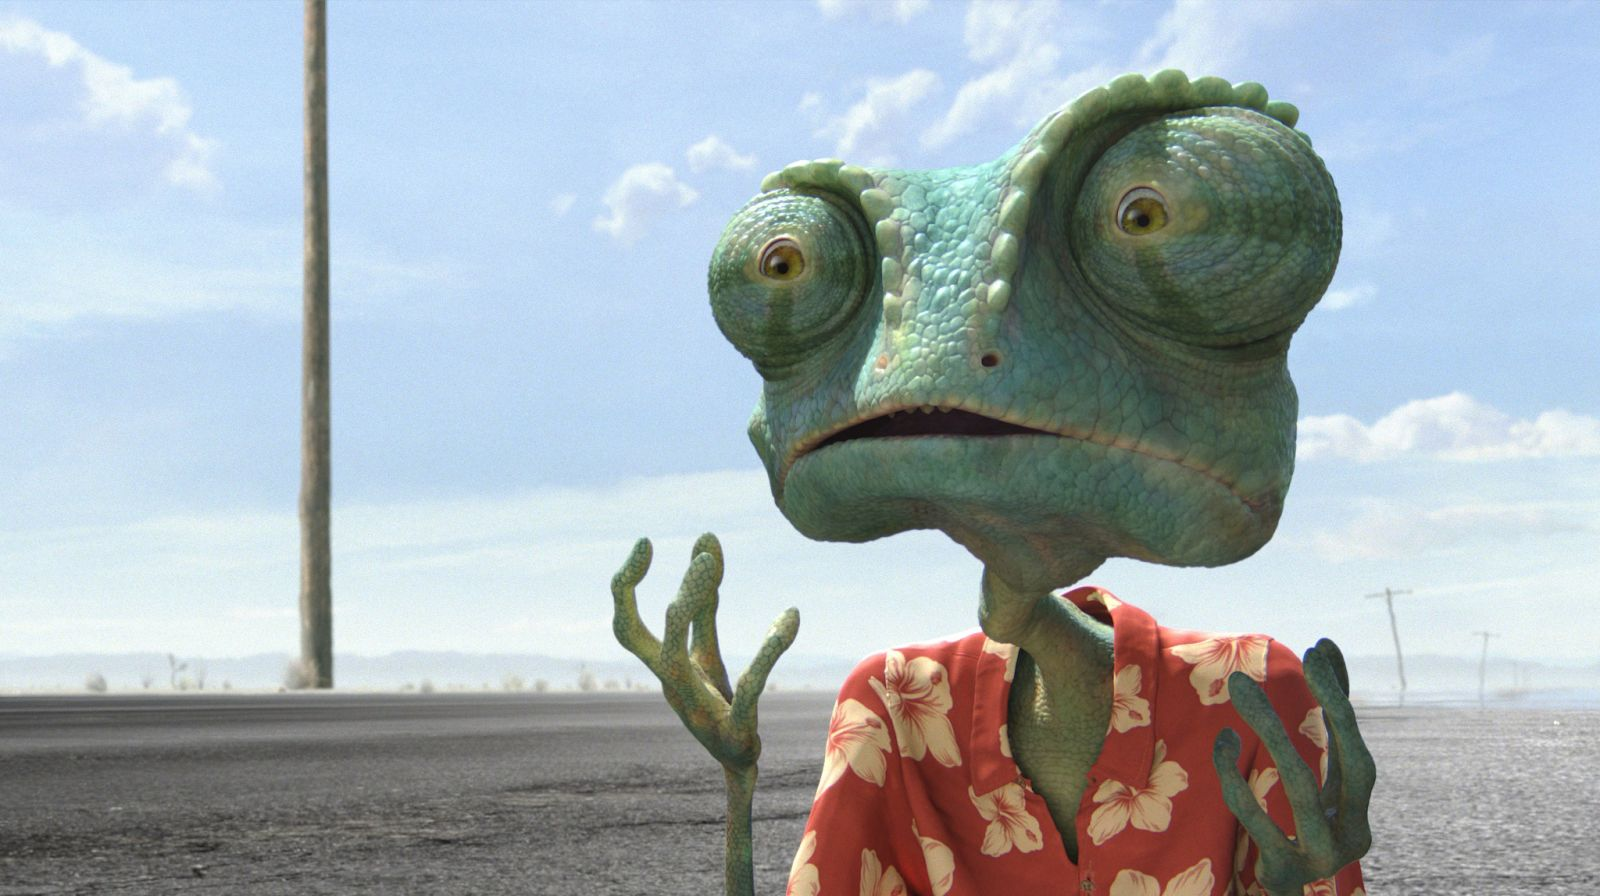
\includegraphics{Figuras-dispersion/Rango.jpg}
\end{frame}

\begin{frame}{Rango}
\protect\hypertarget{rango}{}
Diferencia entre mínimo y máximo, ejemplo:

\(Temp = \{10, 15, 12, 20, 21, 10, 25, 5, 17, 7\}\)

El mínimo es \(5\) y el máximo \(25\)

Rango: \(5, 25\)
\end{frame}

\begin{frame}{Rango intercuartil}
\protect\hypertarget{rango-intercuartil}{}
Diferencia entre \(1^{er}\) y \(3^{er}\) cuartil, ejemplo:

\[Temp = \{5, 7, 10, 10, 12, 15, 17, 20, 21, 25\}\]

\(1^{er}\) cuartil: 10
\end{frame}

\begin{frame}{Desviación estándar}
\protect\hypertarget{desviaciuxf3n-estuxe1ndar}{}
En la literatura estadística se le llama \(\sigma\)

Se calcula con la fórmula:

\[\sigma = \sqrt{\sum_{i = 1}^n \frac{(x_i - \bar{x})^2}{n-1}}\]

Donde \(\bar{x}\), es el promedio de \(X\), y \(n\) es el tamaño de
muestra, o número de observaciones

\(3^{er}\) cuartil: 20

Rango intercuartil: \(10, 20\)
\end{frame}

\begin{frame}{Desviación estándar}
\protect\hypertarget{desviaciuxf3n-estuxe1ndar-1}{}
Se utiliza para medir la distancia promedio entre las observaciones y la
media

Tiene implicaciones directas sobre las mediciones de probabilidad:

El intervalo \(\bar{x} \pm \sigma\) contiene \(\approx 69 \%\) de
observaciones
\end{frame}

\begin{frame}{Desviación estándar, ejemplo}
\protect\hypertarget{desviaciuxf3n-estuxe1ndar-ejemplo}{}
\[Temp = \{5, 7, 10, 10, 12, 15, 17, 20, 21, 25\}\]

\[\bar{Temp} = 15\]

\[\sigma = 6.36\]

\(15 \pm 6.36 = \{8.63, 21.36\}, 7/10= 70\% \approx 69 \%\) de
observaciones están en el intervalo
\end{frame}

\begin{frame}{Varianza}
\protect\hypertarget{varianza}{}
Es derivada de la desviación estándar

Se le llama \(\sigma^2\) es la variación total de la variable de estudio
\end{frame}

\begin{frame}{Reflexión}
\protect\hypertarget{reflexiuxf3n}{}
Rango, rango intercuartil, desviación y varianza:

\begin{itemize}
\item
  Representan variación en mismas unidades, p.~ej.:
\item
  Si \(Temp\) es medida en \(°\mathrm{C}\), \(\sigma_{Temp}\) está en
  \(°\mathrm{C}\)
\end{itemize}
\end{frame}

\begin{frame}{Otras medidas de dispersión}
\protect\hypertarget{otras-medidas-de-dispersiuxf3n}{}
Coeficiente de variación:

\[C_V = \frac{\sigma}{\bar{x}}\]

Es el cociente de la desviación y media

Ejemplo:

\[C_{V, Temp} = \frac{6.36}{15} = 0.42\]

La variación es equivalente al \(42 \%\) de la media
\end{frame}

\end{document}
